\chapter{Az S-gráf modell}
Az S-gráf keretrendszer volt az első publikált gráf elméleten alapuló módszer szakaszos gyártórendszerek ütemezési problémáinak megoldására. \cite{Sanmarti2002}
A keretrendszer egy irányított gráf modellből, az S-gráfból és a hozzá tartozó algoritmusokból áll. \cite{SANMARTI1998S847}
Az S-gráf egy speciális irányított gráf, amely nem csupán a probléma vizualizációjára képes, hanem egy matematikai modell is.
A keretrendszerben a recepteket, valamint a félkész-, illetve a teljes ütemterveket is az S-gráf reprezentálja.
Ezekben a gráfokban a termékeket, illetve a feladatokat a pontok jelölik, amelyeket csomópontoknak (node) nevezünk.
Ezenkívül, ha két feladat között összeköttetés van, ezt a gráfon a két feladatot reprezentáló csomópontok közötti nyíl jelöli.
Az ütemezési információ nélküli S-gráfot \textbf{recept gráfnak} nevezzük, melyre egy példa a \ref{recipeGraph} ábrán látható.
\begin{figure}[H]
\begin{center}
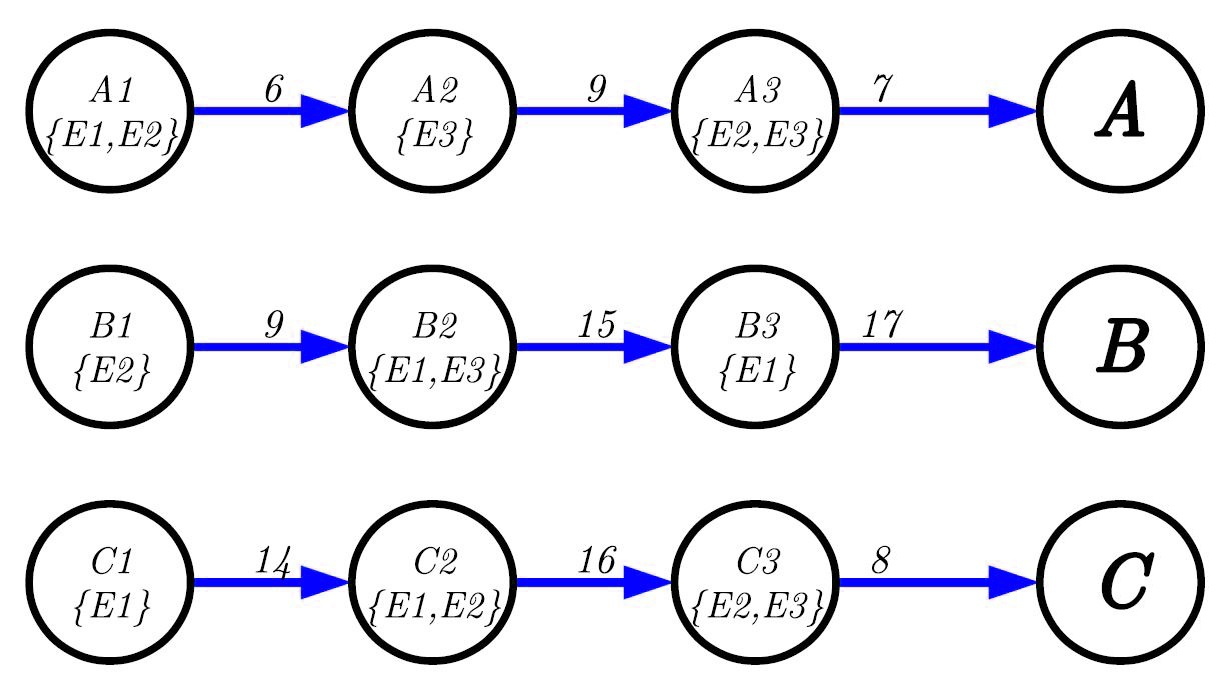
\includegraphics[scale=0.35]{recipeGraph}
\caption{A recept gráf szemléltetése}
\label{recipeGraph}
\end{center}
\end{figure}
\section{Profit maximalizálás S-gráffal} \label{SgraphProfitMax}